\section{Balanced Clustering}
\label{sec:imbalance}

Task clustering has been widely used to address the low performance of very short tasks on platforms where the system overhead is high, such as distributed computing infrastructures. However, techniques do not consider the load balance problem. In particular, merging tasks within a level without considering the runtime variance may cause load imbalance (Runtime Imbalance), or merging without considering data dependency may lead to data locality problems (Dependency Imbalance).

In this section, we introduce metrics that quantitatively capture workflow characteristics to measure runtime and dependence imbalances. We then present methods to handle the load balance problem.

\subsection{Imbalance Metrics}


\textbf{Runtime Imbalance} describes the difference of the task/job runtime of a group of tasks/jobs. In this work, we denote the \textbf{Horizontal Runtime Variance} ($HRV$) as the ratio of the standard deviation in task runtime to the average runtime of tasks/jobs at the same horizontal level of a workflow. At the same horizontal level, the job with the longest runtime often controls the release of the next level jobs. A high $HRV$ value means that the release of next level jobs has been delayed.
Therefore, to improve runtime performance, it is meaningful to reduce the standard deviation of job runtime. Fig.~\ref{fig:imbalance_rv} shows an example of four independent tasks $t_1$, $t_2$, $t_3$ and $t_4$ where task runtime of $t_1$ and $t_2$ is half of that of $t_3$ and $t_4$. In the Horizontal Clustering (HC) approach, a possible clustering result could be merging $t_1$ and $t_2$ into a clustered job and $t_3$ and $t_4$ into another. This approach results in imbalanced runtime, i.e., $HRV > 0$ (Fig.~\ref{fig:imbalance_rv}-top). In contrast, a balanced clustering strategy should try its best to evenly distribute task runtime among jobs as shown in Fig.~\ref{fig:imbalance_rv} (bottom). Generally speaking, a smaller \emph{HRV} means that the runtime of tasks at the same horizontal level is more evenly distributed and therefore it is less necessary to balance the runtime distribution. However, runtime variance is not able to describe how regular is the structure of the dependencies between the tasks.

\begin{figure}[htb]
	\centering
	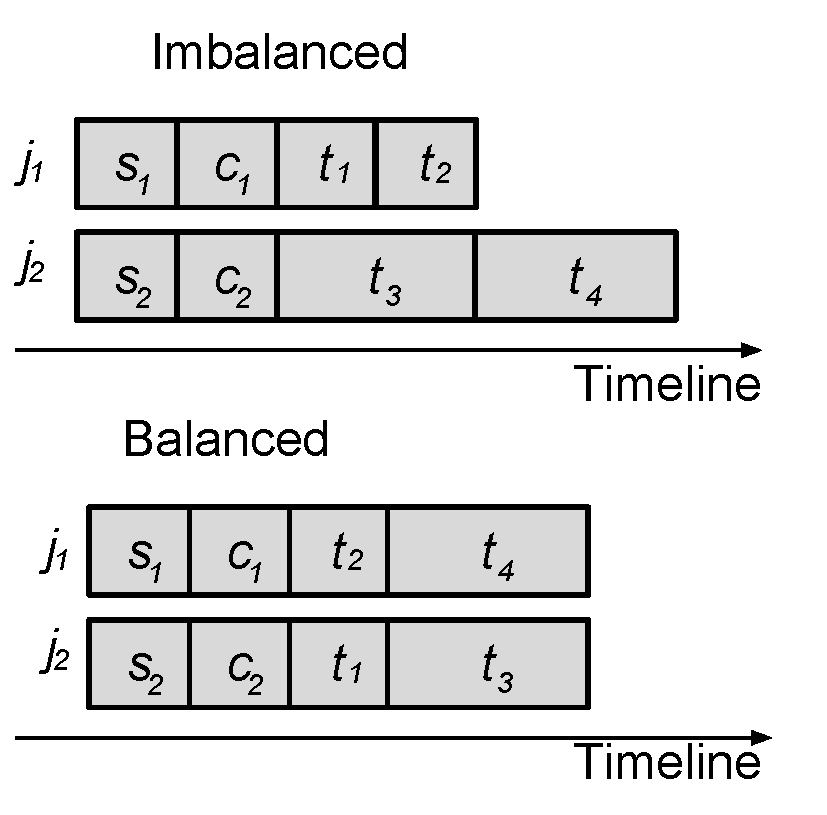
\includegraphics[width=0.6\linewidth]{figures/imbalance/rv.pdf}
	\captionof{figure}{An Example of Runtime Variance.}
	\label{fig:imbalance_rv}
\end{figure}




%is the second reason why we need to use balanced clustering and it

\textbf{Dependency Imbalance} means that the task clustering at one horizontal level forces the tasks at the next level (or even subsequent levels) to have severe data locality problem and thus loss of parallelism. For example, in Fig.~\ref{fig:imbalance_dv}, we show a two-level workflow composed of four tasks in the first level and two in the second. Merging $t_1$ with $t_2$ and $t_3$ with $t_4$ (imbalanced workflow in Fig.~\ref{fig:imbalance_dv}) forces $t_5$ and $t_6$ to transfer files from two locations and wait for the completion of $t_1$, $t_2$, $t_3$, and $t_4$.  A balanced clustering strategy groups tasks that have the maximum number of child tasks in common. Thus, $t_5$ can start to execute as soon as $t_1$ and $t_3$ are completed, and so can $t_6$. To measure and quantitatively demonstrate the Dependency Imbalance of a workflow, we propose two  metrics: ($i$) Impact Factor Variance, and ($ii$) Distance Variance. 

\begin{figure}[htb]
	\centering
	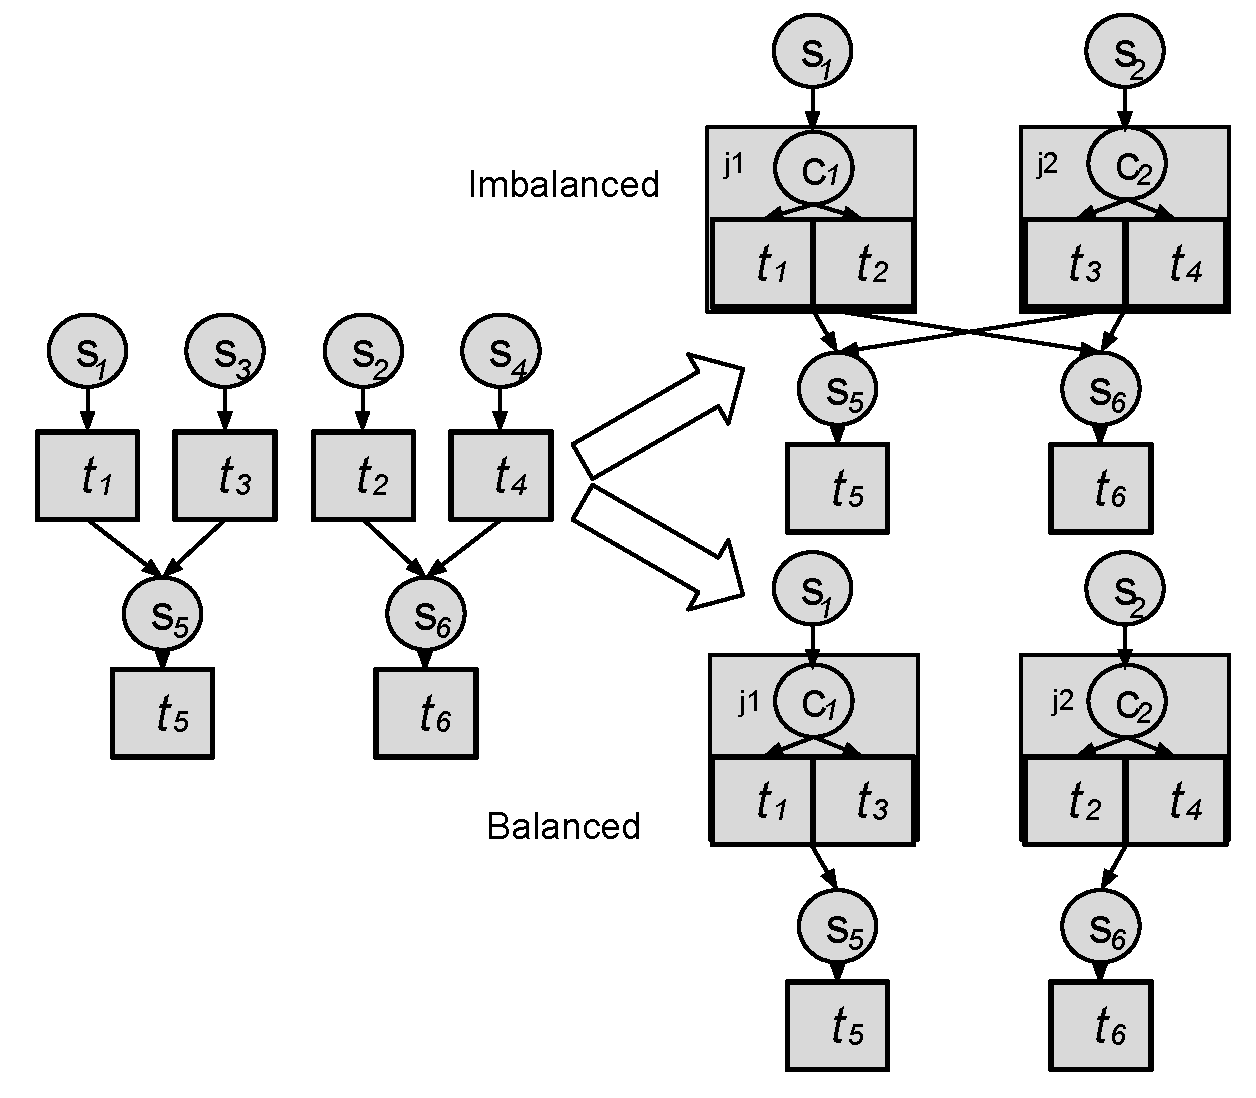
\includegraphics[width=\linewidth]{figures/imbalance/dv.pdf}
	\captionof{figure}{An Example of Dependency Variance.}
	\label{fig:imbalance_dv}
\end{figure}

We define the \textbf{Impact Factor Variance} ($IFV$) of tasks as the standard deviation of their impact factor. The intuition behind the Impact Factor is that we aim to capture the similarity of tasks/jobs in a graph by measuring their relative impact factor or importance to the entire graph. Intuitively speaking, tasks with similar impact factors should be merged together compared to tasks with different impact factors. Also, if all the tasks have similar impact factors, the workflow structure tends to be more `even' or `regular'. The \textbf{Impact Factor} ($IF$) of a task $t_u$ is defined as follows:

%We first define the \textbf{Impact Factor} ($IF$) of a task in a recursive way as below. 

\begin{equation}
\label{eq:imbalance_impact_factor}
	IF(t_u)=\sum_{t_v\in Child(t_u)}^{}\frac{IF(t_v)}{||Parent(t_v)||}
\end{equation}
where $Child(t_u)$ denotes the set of child tasks of $t_u$, and $||Parent(t_v)||$ the number of parent tasks of $t_v$. For simplicity, we assume the $IF$ of a workflow exit task (e.g. $t_5$ in Fig.~\ref{fig:imbalance_dv}) as 1.0. For instance, consider the two workflows presented in Fig.~\ref{fig:imbalance_hifv}. $IF$ for $t_1$, $t_2$, $t_3$, and $t_4$ are computed as follows:

\begin{eqnarray}
	\displaystyle  
	&IF(t_7 )=1.0, IF(t_6 )=IF(t_5 )=IF(t_7 )/2=0.5\nonumber  \\
	&IF(t_1 )=IF(t_2 )=IF(t_5 )/2=0.25\nonumber \\
	&IF(t_3 )=IF(t_4 )=IF(t_6 )/2=0.25\nonumber 
\end{eqnarray}
Thus, IFV($t_1$, $t_2$, $t_3$, $t_4$) = 0. In contrast, $IF$ for $t_1'$, $t_2'$, $t_3'$, and $t_4'$ are:

\begin{eqnarray}
	\displaystyle  
	&IF(t_7')=1.0, IF(t_6')=IF(t_5')=IF(t_1')=IF(t_7')/2=0.5\nonumber \\
	&IF(t_2')=IF(t_3')=IF(t_4')=IF(t_6')/3=0.17 \nonumber
\end{eqnarray}
Therefore, the $IFV$ value for {$t_1'$, $t_2'$, $t_3'$, $t_4'$} is 0.17, which means it is less regular than the workflow in Fig.~\ref{fig:imbalance_hifv} (left). In this work, we use \textbf{HIFV} (Horizontal IFV) to indicate the $IFV$ of tasks at the same horizontal level. The time complexity of calculating all the $IF$ of a workflow with $n$ tasks is $O(n)$.  



\begin{figure}[htb]
	\centering
	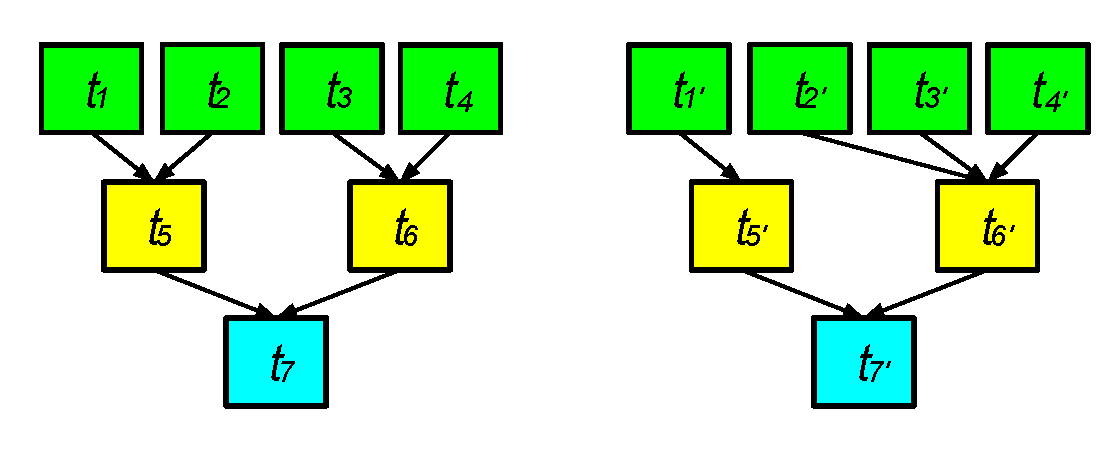
\includegraphics[width=0.85\linewidth]{figures/imbalance/dependency.pdf}
	\captionof{figure}{Example of workflows with different data dependencies.}
	\label{fig:imbalance_hifv}
\end{figure}
% In Fig~\ref{fig:hifv}, the left workflow should have a smaller Dependency Imbalance problem than the right workflow since the dependencies in the left figure are more repetitive and regular. We define the \textbf{Impact Factor Variance} ({\em IFV}) of tasks to be the standard deviation of their $IF$. Therefore, the {\em IFV} of {$t_1$, $t_2$, $t_3$, $t_4$} is 0. In contrast, for the workflow in Fig~\ref{fig:hifv} (Right), we have:

\textbf{Distance Variance} ($DV$) describes how `closely' tasks are to each other. The distance between two tasks/jobs is defined as the cumulative length of the path to their closest common successor. If they do not have a common successor, the distance is set to infinity. For a group of $n$ tasks/jobs, the distance between them is represented by a $n \times n$ matrix $D$, where an element $D(u,v)$ denotes the distance between a pair of tasks/jobs $u$ and $v$. For any workflow structure, $D(u,v)=D(v,u)$ and $D(u,u)=0$, thus we ignore the cases when $u \geq v$. Distance Variance is then defined as the standard deviation of all the elements $D(u,v)$ for $u<v$. The time complexity of calculating all the $D$ of a workflow with $n$ tasks is $O(n^2)$. 

Similarly, $HDV$ indicates the $DV$ of a group of tasks/jobs at the same horizontal level. For example, Table~\ref{tab:imblance_metric} shows the distance matrices of tasks from the first level for both workflows of Fig.~\ref{fig:imbalance_hifv} ($D_1$ for the workflow in the left and $D_2$ for the workflow in the right). $HDV$ for $t_1, t_2, t_3$, and $t_4$ is 1.03, and for $t_1', t_2', t_3'$, and $t_4'$ is 1.10. In terms of distance variance, $D_1$ is more `even' than $D_2$. Intuitively speaking, a smaller $HDV$ means the tasks at the same horizontal level are more equally `distant' to each other and thus the workflow structure tends to be more `evenly' and `regular'. 

In conclusion, runtime variance and dependency variance offer a quantitative and comparable tool to measure and evaluate the internal structure of a workflow. 


\begin{table}[htb]
	\footnotesize
	\centering
	\begin{tabular}{l|rrrr}
		$D_1$ & $t_1$ & $t_2$ & $t_3$ &$t_4$\\
		\hline
		$t_1$ & 0 & 2 & 4 & 4 \\
		$t_2$ & 2 & 0 & 4 & 4 \\
		$t_3$ & 4 & 4 & 0 & 2\\
		$t_4$ & 4 & 4 & 2 & 0 \\
	\end{tabular}
	\quad
	\begin{tabular}{l|rrrr}
		$D_2$ & $t_1'$ & $t_2'$ & $t_3'$ &$t_4'$\\
		\hline
		$t_1'$ & 0 & 4 & 4 & 4 \\
		$t_2'$ & 4 & 0 & 2 & 2 \\
		$t_3'$ & 4 & 2 & 0 & 2\\
		$t_4'$ & 4 & 2 & 2 & 0 \\
	\end{tabular}
	\caption{Distance matrices of tasks from the first level of workflows in Fig.~\ref{fig:imbalance_hifv}.}
	\label{tab:imblance_metric}
\end{table}


\subsection{Balanced Clustering Methods}
\label{sec:methods}
In this subsection, we introduce our balanced clustering methods used to improve the runtime balance and dependency balance in task clustering. We first introduce the basic runtime-based clustering method and then two other balancing methods that address the dependency imbalance problem. We use the metrics presented in the previous subsection to evaluate a given workflow to decide which balancing method(s) is(are) more appropriate. 

Algorithm~\ref{alg:imbalance_algo} shows the pseudocode of our balanced clustering algorithm that uses a combination of these balancing methods and metrics.  The maximum number of clustered jobs (size of $CL$) is equal to the number of available resources multiplied by a \emph{clustering factor}. 
%We compare the performance of using different \emph{clustering factor} in Section 5. 

\begin{algorithm}[htb]
	\caption{ Balanced Clustering algorithm}
	\footnotesize
	\label{alg:imbalance_algo}
	\begin{algorithmic}[1]
		\Require $W$: workflow; $CL$: list of clustered jobs; $C$: the required size of $CL$; 
		\Ensure The job runtime of $CL$ are as even as possible
		\Procedure{Clustering}{$W,D,C$}
			\State Sort $W$ in decreasing order of the size of each level
			\For{$level < $the depth of $W$}
				\State $TL\gets $\ \Call{GetTasksAtLevel}{$w,level$} \Comment{Partition $W$ based on depth}
				\State $CL\gets$  \ \Call{Merge}{$TL,C$} \Comment{Form a list of clustered jobs}
				\State $W \gets W - TL + CL$  \Comment{Merge dependencies as well} 
			\EndFor
		\EndProcedure
		\Procedure{Merge}{$TL, C$}
			\State Sort $TL$ in decreasing order of task runtime
			\For{$t\ in\ TL$}
				\State $J \gets $\ \Call{GetCandidateJob}{$CL, t$} \Comment{Get a candidate task}
				\State  $J \gets J\ +\ t$ \Comment{Merge it with the clustered job}
			\EndFor
			\State \textbf{return} $CL$
		\EndProcedure
		\Procedure{GetCandidateJob}{$CL, t$}
			\State Selects a job based on balanced clustering methods
		\EndProcedure
	\end{algorithmic}
\end{algorithm}

We examine tasks in a level-by-level approach starting from the level with the largest width (number of tasks at the same level, \texttt{line 2}). The intuition behind this breadth favored approach is that we believe it should improve the performance most. Then, we determine which type of imbalance problem a workflow experiences based on the balanced clustering metrics presented previously ($HRV$, $HIFV$, and $HDV$), and accordingly, we select a combination of balancing methods. \textsc{GetCandidateJob} selects a job (\texttt{line 12}) from a list of potential candidate jobs ($CL$) to be merged with the targeting task ($t$). Below we introduce the three balancing methods proposed in this work.

\textbf{Horizontal Runtime Balancing} (HRB) aims to evenly distribute task runtime among jobs. Tasks with the longest runtime are added to the job with the shortest runtime. This greedy method is used to address the imbalance problem caused by runtime variance at the same horizontal level. Fig.~\ref{fig:imbalance_hrb} shows how HRB works in an example of four jobs with different job runtime (assuming the height of a job is its runtime). For the given task ($t_0$), HRB sorts the potential jobs ($j_1$, $j_2$, $j_3$, and $j_4$) based on their runtime and selects the shortest job (in this case $j_1$ or $j_2$). 

\begin{figure}[htb]
	\centering
	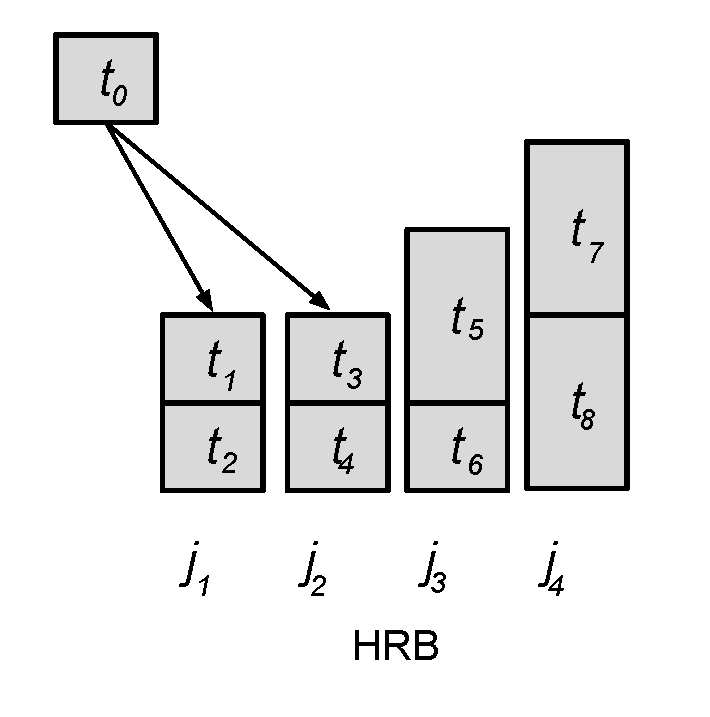
\includegraphics[width=0.5\linewidth]{figures/imbalance/algorithm_hrb.pdf}
	\caption{An example of HRB.}
	\label{fig:imbalance_hrb}
\end{figure}

However, HRB may cause a dependency imbalance problem since the clustering does not take data dependency into consideration. To address this problem, we propose the \textbf{Horizontal Impact Factor Balancing} (HIFB) and the \textbf{Horizontal Distance Balancing} (HDB) methods. 

In HRB, candidate jobs are sorted by their runtime, while in HIFB jobs are first sorted based on their similarity of $IF$, then on runtime. For example, in Fig.~\ref{fig:imbalance_hifb}, assuming 0.2, 0.2, 0.1, and 0.1 IF values of $j_1$, $j_2$, $j_3$, and $j_4$ respectively, HIFB selects a list of candidate jobs with the same IF value, i.e. $j_3$ and $j_4$. Then, HRB is performed to select the shortest job ($j_3$). 

\begin{figure}[htb]
	\centering
	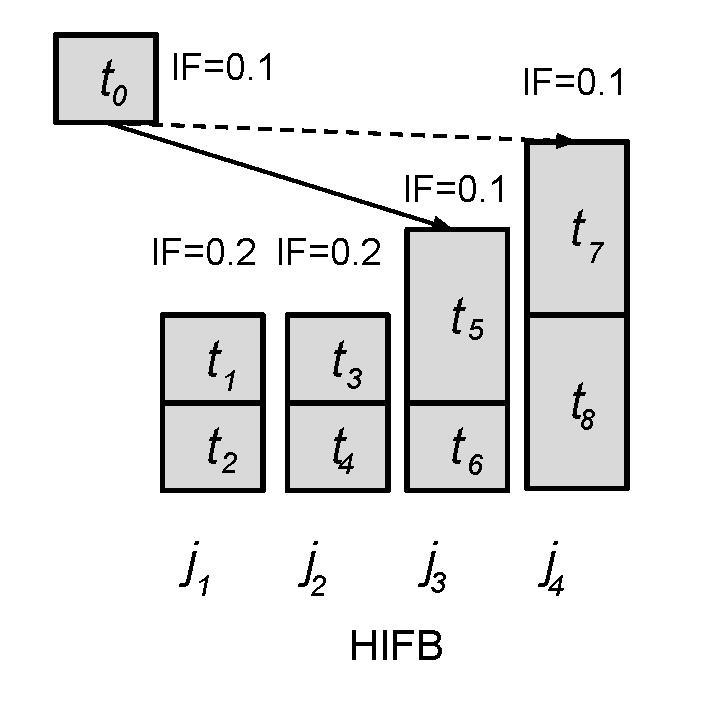
\includegraphics[width=0.5\linewidth]{figures/imbalance/algorithm_hifb.pdf}
	\captionof{figure}{An example of HIFB.}
	\label{fig:imbalance_hifb}
\end{figure}

Similarly, in HDB jobs are sorted based on the distance between them and the targeted task $t_0$, then on their runtimes. For instance, in Fig.~\ref{fig:imbalance_hdb}, assuming 2, 4, 4, and 2 the distances to $j_1$, $j_2$, $j_3$, and $j_4$ respectively, HDB selects a list of candidate jobs with the minimal distance ($j_1$ and $j_4$). Then, HRB is performed to select the shortest job ($j_1$). 

\begin{figure}[htb]
	\centering
	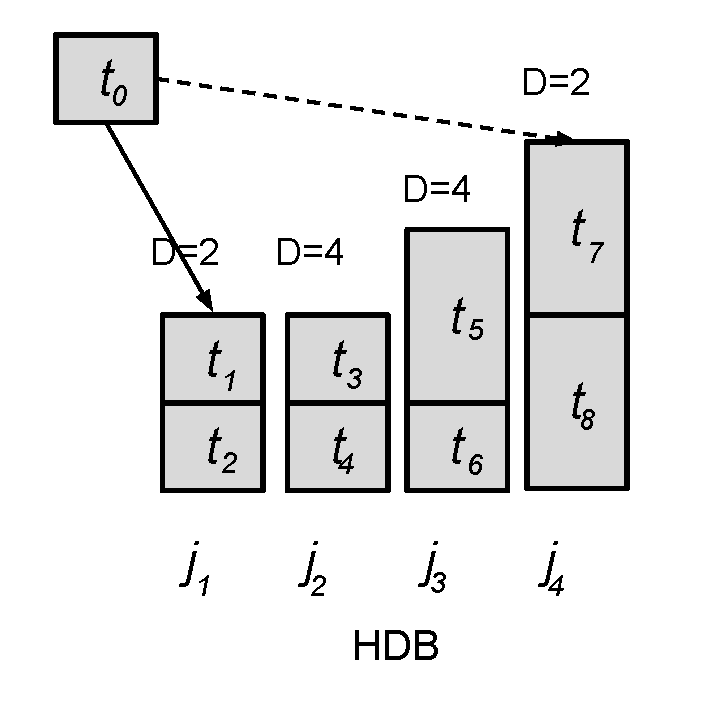
\includegraphics[width=0.5\linewidth]{figures/imbalance/algorithm_hdb.pdf}
	\captionof{figure}{An example of HDB.}
	\label{fig:imbalance_hdb}
\end{figure}

In conclusion, these balancing methods have different preference on the selection of a candidate job to be merged with the targeting task. HIFB tends to group tasks that share similar position/importance to the workflow structure. HDB tends to group tasks that are closed to each other to reduce data transfers. 
%Table~\ref{tab:2} summarizes the imbalance metrics and balancing methods presented in this work. 

%\begin{figure}[htb]
%	\centering
%	\begin{tabular}{l|l}
%		\hline
%		Imbalance Metrics & $abbr.$   \\
%		\hline
%		Horizontal Runtime Variance & \emph{HRV}   \\ 
%		%Pipeline Runtime Variance &{\em PRV}  \\ 
%		Horizontal Impact Factor Variance & \emph{HIFV} \\ 
%		Horizontal Distance Variance & \emph{HDV}  \\ 
%		\hline
%		Balancing Methods & $abbr.$  \\
%		\hline
%		Horizontal Runtime Balancing & HRB   \\ 
%		% Vertical Clustering & VC \\ 
%		Horizontal Impact Factor Balancing & HIFB\\ 
%		Horizontal Distance Balancing & HDB \\ 
%		\hline
%	\end{tabular}
%	\captionof{table}{Imbalance metrics and balancing methods.}
%	\label{tab:2}
%	\vspace{-10pt}
%\end{figure}

